% Begin the document and set up the style of the document
\documentclass[a4paper]{article}

% Install the required packages for the document 
\usepackage{envmath}
\usepackage{esvect}
\usepackage{graphicx}
\usepackage{gensymb}
\usepackage{tikz}
\usepackage{geometry}
\usepackage{enumitem}
\usepackage{mathtools}
\usepackage{graphicx}
\usepackage{amsmath}
\usepackage{amscd}
\usepackage{amssymb}
\usepackage{amsfonts}
\usepackage{pgf}
\usepackage{tikz}
\usepackage{mathrsfs}
\usepackage{asyalign}
\usepackage{physics}
\usepackage{cite}
\usepackage{url}
\usepackage[tableposition=top]{caption}
\usepackage{ifthen}
\usepackage[utf8]{inputenc}
\usetikzlibrary{arrows}

% Page and style settings
\parskip=8pt
\parindent=0pt
% Right margin
\textwidth=6.25in
% Left margin
\oddsidemargin=0pt
\evensidemargin=0pt
% Bottom margin
\textheight=10in
% Top margin
\topmargin=-0.75in
\baselineskip=11pt
% end of page and other style settings

\renewcommand{\familydefault}{\sfdefault}

% Begin the text of the document
\begin{document}

% Page numbering
\pagenumbering{arabic}
% the following four lines force that lines break after 80 characters in the R-output

% Begin title and formatting
\begin{center}
{\large \textbf{MATH 1906 - Differential Calculus SSP}}\\
\end{center}

% Table formatting and text
\vspace{-1mm}
\begin{tabular*}{1.0\linewidth}{@{\extracolsep{\fill}}lr@{}}
  \hline\noalign{\smallskip}
Semester 1, \the\year & Name = \texttt{Keegan Gyoery} \\ 
Tutor = \texttt{Daniel Daners} & SID = \texttt{470413467} \\
\hline
\end{tabular*}

% Centre the heading for the document 
\begin{center}
 \large \textbf{Assignment 1 - Maps}\\
\end{center}

%%%%%%%%%%%%%%%%%%%%%%%%%%%%%%%%%%%%%%%
%%%%%%%%%%%%%%%%%%%%%%%%%%%%%%%%%%%%%%%
%%%%%%%%%%%%%%%%%%%%%%%%%%%%%%%%%%%%%%%
%%%%%%%%%%%%%%%%%%%%%%%%%%%%%%%%%%%%%%%

% Begin the list for the question parts
\begin{enumerate}[label=(\alph*)]
	
	% The first item on the list - part a question
	\item Using an equal area map projection, we are required to prove that $b^2cos\theta = 2v\frac{dv}{d\theta}$. In order to do this we need to examine the area on the sphere and secondly on the map projection, to derive the above relationship.

	Now we know that the gradient of the border lines of the map projection is $\pm \frac{b}{a}$. Furthermore we are given that the total area of the map projection is equal to the surface area of the sphere. 

	% Display the equation to solve for the surface area of the sphere in terms of the map projection area.
	\begin{align*}
	4\pi R^2 & = \frac{1}{2}(2a)(b) + \frac{1}{2}(2a)(b)\\
	& = ab + ab\\
	& = 2ab\\
	\therefore 4\pi & = 2ab\\
	\therefore 2\pi & = ab\\
	\end{align*}

	Examining the sphere, with radius 1 and centered on the origin, we will need to examine the area of a strip that is created by the difference in the latitudes $\theta$ and $\theta + \Delta\theta$. The area of the strip is given by integrating the circumference from $\theta$ to $\theta + \Delta\theta$. The radius of the latitude $\theta$ is given by $\cos{\theta}$.

	% Display the image of the sphere
	\begin{center}
	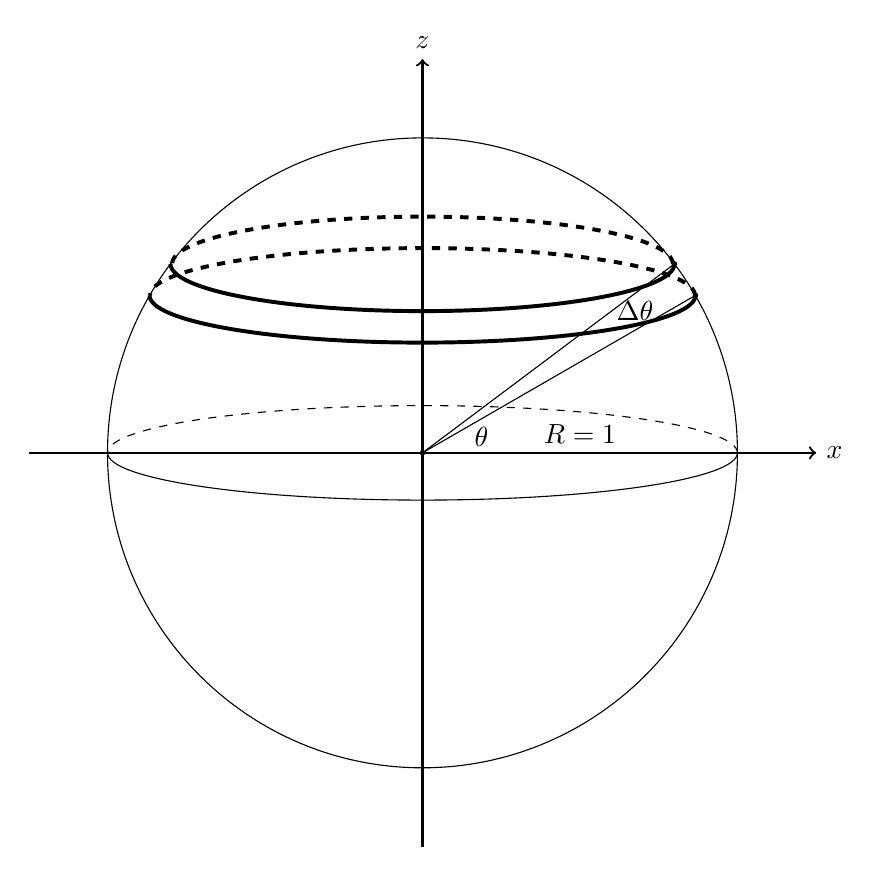
\begin{tikzpicture}
		% X - axis
		\draw[->,thick] (-5,0)--(5,0) node[right]{$x$};
		% Y - axis
		\draw[->,thick] (0,-5)--(0,5) node[above]{$z$};
	  	% Top Latitude arc
	  	\draw[line width = 0.5mm] (-3.20,2.4) arc (180:360:3.20 and 0.6);
	  	% Top Latitude arc dashed
	  	\draw[dashed][line width = 0.5mm] (3.18,2.4) arc (0:180:3.18 and 0.6);
	  	% Bottom Latitude arc
	  	\draw[line width = 0.5mm] (-3.467,2.0) arc (180:360:3.467 and 0.6);
	  	% Bottom Latitude arc dashed
	  	\draw[dashed][line width = 0.5mm] (3.46,2.0) arc (0:180:3.46 and 0.6);
	  	% Fill point for b lat
	  	\fill[fill=black] (3.467,2.0) circle (1pt);
	  	% Fill point for t lat
	  	\fill[fill=black] (3.20,2.4) circle (1pt);
	  	% Line to b lat
	  	\draw (0,0 ) -- (3.467,2.0);
	 	% Line to t lat
	 	\draw (0,0 ) -- (3.20,2.4);
	  	% Label the delta theta angle
	  	\node at (2.7, 1.8) {$\Delta \theta$};
	  	% Label the theta angle
	  	\node at (0.75, 0.2) {$\theta$};
	  	% Circle
	  	\draw (0,0) circle (4cm);
	  	% Center arc
	  	\draw (-4,0) arc (180:360:4 and 0.6);
	  	% Center arc dashed
	  	\draw[dashed] (4,0) arc (0:180:4 and 0.6);
	  	% Fill point at center
	  	\fill[fill=black] (0,0) circle (1pt);
	  	% Radius dashed
	  	\draw[dashed] (0,0 ) -- node[above]{$R = 1$} (4,0);
	\end{tikzpicture}
	\end{center}

	% Display the equation to solve for the surface area of the strip on the sphere
	\begin{align*}
	A_{strip_{sphere}} & = \int_{\theta}^{\theta + \Delta \theta} 2\pi \cos \theta d\theta\\
	& = 2\pi \int_{\theta}^{\theta + \Delta \theta} \cos{\theta} d\theta\\
	& = 2\pi \Big[\sin(\theta + \Delta \theta) - \sin(\theta)\Big]\\
	& = ab \Big[\sin(\theta + \Delta \theta) - \sin(\theta)\Big]\\
	\end{align*}

	Now considering a strip on the map projection, we will find the area using the area of the triangles that bound the strip on the map projection. Considering the triangles that lie to the right of the y-axis, we will label the base length of the larger triangle as $a_2$, and the base length of the smaller triangle as $a_1$. Thus the area of each triangle is given by:

	\begin{center}
	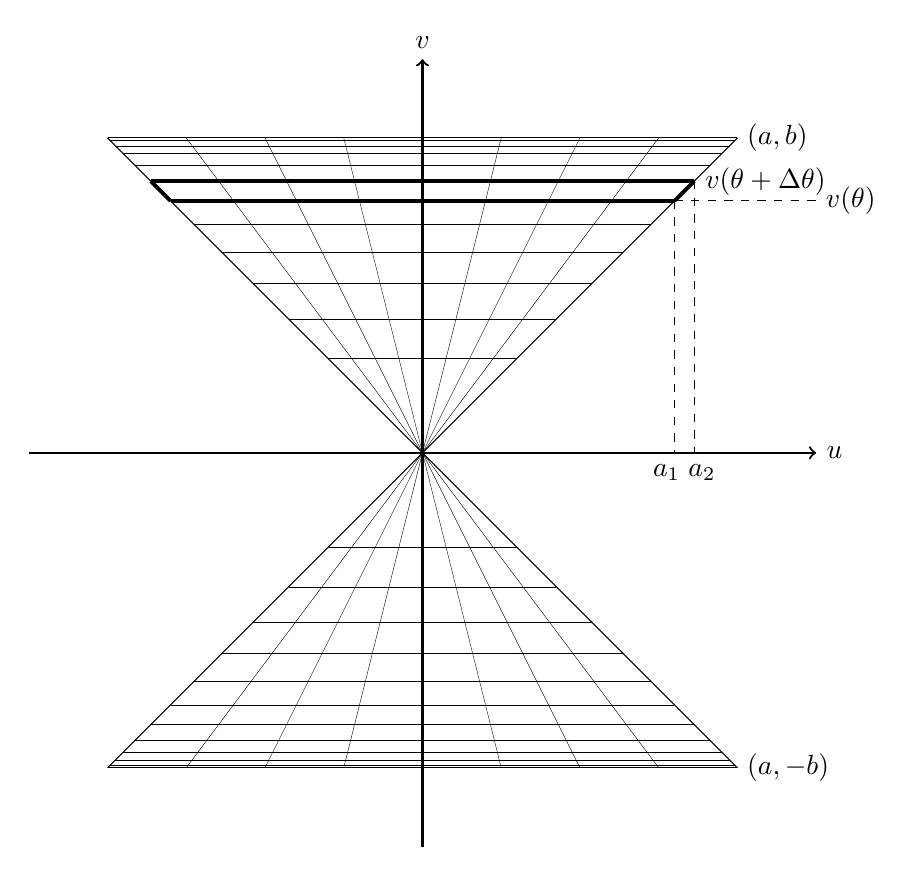
\begin{tikzpicture}
		% X - axis
		\draw[->,thick] (-5,0)--(5,0) node[right]{$u$};
		% Y - axis
		\draw[->,thick] (0,-5)--(0,5) node[above]{$v$};
		% Lines for the meridians right side
		\draw (-4,-4 ) -- (4,4);
		\draw [line width=0.05mm] (-3,-4 ) -- (3,4);
		\draw [line width=0.05mm] (-2,-4 ) -- (2,4);
		\draw [line width=0.05mm] (-1,-4 ) -- (1,4);
		\draw [line width=0.05mm] (0,-4 ) -- (0,4);
		\draw [line width=0.05mm] (1,-4 ) -- (-1,4);
		\draw [line width=0.05mm] (2,-4 ) -- (-2,4);
		\draw [line width=0.05mm] (3,-4 ) -- (-3,4);
		\draw (4,-4 ) -- (-4,4);
		\draw (-4,4 ) -- (4,4) node[right]{$(a,b)$};
		\draw (-4,-4 ) -- (4,-4) node[right]{$(a,-b)$};
		% Draw latitude lines
		\draw [line width=0.05mm] (-3.965,3.965) -- (3.965,3.965);
		\draw [line width=0.05mm] (-3.9,3.9) -- (3.9,3.9);
		\draw [line width=0.05mm] (-3.8,3.8) -- (3.8,3.8);
		\draw [line width=0.05mm] (-3.65,3.65) -- (3.65,3.65);
		\draw [line width=0.5mm] (-3.45,3.45) -- (3.45,3.45) node[right]{$v(\theta + \Delta \theta)$};
		\draw [line width=0.5mm] (-3.2,3.2) -- (3.2,3.2);
		\draw [line width=0.05mm] (-2.9,2.9) -- (2.9,2.9);
		\draw [line width=0.05mm] (-2.55,2.55) -- (2.55,2.55);
		\draw [line width=0.05mm] (-2.15,2.15) -- (2.15,2.15);
		\draw [line width=0.05mm] (-1.7,1.7) -- (1.7,1.7);
		\draw [line width=0.05mm] (-1.2,1.2) -- (1.2,1.2);
		% Bolding the strip
		\draw [line width=0.5mm] (3.2,3.2) -- (3.45,3.45);
		\draw [line width=0.5mm] (-3.2,3.2) -- (-3.45,3.45);
		% Nodes and labels on the graph
		\draw[dashed] (3.45,3.45) -- (3.45,0);
		\node at (3.55,-0.25) {$a_2$};
		\draw[dashed] (3.2,3.2) -- (3.2,0);
		\node at (3.10,-0.25) {$a_1$};
		\draw[dashed] (3.2,3.2) -- (5,3.2) node[right]{$v(\theta)$};
		% Lines for the meridians left side
		\draw [line width=0.05mm] (-3.965,-3.965) -- (3.965,-3.965);
		\draw [line width=0.05mm] (-3.9,-3.9) -- (3.9,-3.9);
		\draw [line width=0.05mm] (-3.8,-3.8) -- (3.8,-3.8);
		\draw [line width=0.05mm] (-3.65,-3.65) -- (3.65,-3.65);
		\draw [line width=0.05mm] (-3.45,-3.45) -- (3.45,-3.45);
		\draw [line width=0.05mm] (-3.2,-3.2) -- (3.2,-3.2);
		\draw [line width=0.05mm] (-2.9,-2.9) -- (2.9,-2.9);
		\draw [line width=0.05mm] (-2.55,-2.55) -- (2.55,-2.55);
		\draw [line width=0.05mm] (-2.15,-2.15) -- (2.15,-2.15);
		\draw [line width=0.05mm] (-1.7,-1.7) -- (1.7,-1.7);
		\draw [line width=0.05mm] (-1.2,-1.2) -- (1.2,-1.2);

	\end{tikzpicture}
	\end{center}

	% Display the equation and solve for the area of each triangle
	\begin{align*}
	A_1 & = \frac{1}{2}a_{1}v(\theta)\\
	A_2 & = \frac{1}{2}a_{2}v(\theta + \Delta \theta)\\
	\end{align*}

	Thus the area of the strip is given by subtracting the total area of the smaller triangle from the larger triangle. The total area is given by twice the above area for each triangle as we only considered half the total area originally.

	% Display the equation and solve for the total area of each trinagle
	\begin{align*}
	A_{1_T} & = a_{1}v(\theta)\\
	A_{2_T} & = a_{2}v(\theta + \Delta \theta)\\
	\end{align*}

	Now considering the equation of the lines that bound the map projection we can determine the values of $a_1$ and $a_2$.

	% Display the equation and solve for the general form of the bounding lines
	\begin{align*}
	y & = mx+b\\
	\therefore y & = \pm \frac{b}{a}x + 0\\
	\end{align*}

	For the values of $a_1$ and $a_2$, we will consider the positive value of the gradient.

	% Display the equation and solve for the values of a1 and a2
	\begin{align*}
	y & = \frac{b}{a}x\\
	\therefore v(\theta) & = \frac{b}{a}{a_1}\\
	\therefore a_1 & = \frac{a}{b}v(\theta)\\
	\therefore v(\theta + \Delta \theta) & = \frac{b}{a}{a_2}\\
	\therefore a_2 & = \frac{a}{b}v(\theta + \Delta \theta)\\
	\therefore A_{1_T} & = a_{1}v(\theta)\\
	& = \frac{a}{b}v(\theta)v(\theta)\\
	\therefore A_{2_T} & = a_{2}v(\theta + \Delta \theta)\\
	& = \frac{a}{b}v(\theta + \Delta \theta)v(\theta + \Delta \theta)\\
	\end{align*}

	Now in order to determine the area of the strip we will subtract the area of the smaller triangle from the area of the larger triangle.

	% Display the eqaution and solve for the value of the area of the strip on the hourglass projection
	\begin{align*}
	A_{strip_{map}} & = A_{2_T} - A_{1_T}\\
	& = \frac{a}{b}v(\theta + \Delta \theta)v(\theta + \Delta \theta) - \frac{a}{b}v(\theta)v(\theta)\\
	& = \frac{a}{b}\bigg[\Big[{v(\theta + \Delta \theta)\Big]^2} - \Big[{v(\theta)}\Big]^2\bigg]\\
	\end{align*}

	As the map projection is by definition an equal area map, we can equate the area on the globe to the area on the map projection. Thus the following relationship can be derived:

	% Display the equatin to solve for the area of the strip on the map and the sphere to prove the required relationship given by the question
	\begin{align*}
	A_{strip_{sphere}} & = A_{strip_{map}}\\
	\therefore ab \Big[\sin(\theta + \Delta \theta) - \sin(\theta)\Big] & = \frac{a}{b}\bigg[\Big[{v(\theta + \Delta \theta)\Big]^2} - \Big[{v(\theta)}\Big]^2\bigg]\\
	\therefore b^2\Big[\sin(\theta + \Delta \theta) - \sin(\theta)\Big] & = \Big[{v(\theta + \Delta \theta)\Big]^2} - \Big[{v(\theta)}\Big]^2\\
	\therefore b^2\frac{\Big[\sin(\theta + \Delta \theta) - \sin(\theta)\Big]}{\Delta \theta} & = \frac{\Big[{v(\theta + \Delta \theta)\Big]^2} - \Big[{v(\theta)}\Big]^2}{\Delta \theta}\\
	\end{align*}

	Now taking the limit as $\Delta \theta \to 0$, we can derive the required result, as we are using the definition of differentiation from first principles.

	% Display the equation to solve for the required expression
	\begin{align*}
	\lim_{{\Delta \theta}\to 0} b^2\frac{\Big[\sin(\theta + \Delta \theta) - \sin(\theta)\Big]}{\Delta \theta} & = \lim_{{\Delta \theta}\to 0} \frac{\Big[{v(\theta + \Delta \theta)\Big]^2} - \Big[{v(\theta)}\Big]^2}{\Delta \theta}\\
	\therefore b^2\frac{d}{d\theta}\Big[\sin(\theta)\Big] & = \frac{d}{d\theta}\bigg[\Big[v(\theta)\Big]^2\bigg]\\
	\therefore b^2{\cos \theta} & = 2v(\theta)\frac{d}{d\theta}\Big[v(\theta)\Big]\\
	\therefore b^2{\cos \theta} & = 2v\frac{dv}{d\theta}\\
	\end{align*}

	Thus we have proved the required result.

	\item From part (a), we have a differential equation, which we can use to solve for $v$ as a funtion of $\theta$.

	% Display the eqaution to solve for v as a function of theta
	\begin{align*}
	b^2{\cos \theta} & = 2v\frac{dv}{d\theta}\\
	\therefore b^2{\cos \theta}{d\theta} & = 2vdv\\
	\therefore \int{b^2{\cos \theta}{d\theta}} & = \int{2vdv}\\
	\therefore b^2\int{{\cos \theta}{d\theta}} & = 2\int{vdv}\\
	\therefore b^2{\sin \theta} + c_1 & = v^2 + c_2\\
	\therefore b^2{\sin \theta} & = v^2 + C\\
	\end{align*}

	Now in order to determine the value of $C$, we will use the value of $\theta = 0$ and thus $v=0$.

	% Display the equation to solve for the value of C
	\begin{align*}
	b^2{\sin \theta} & = v^2 + C\\
	b^2{\sin 0} & = 0^2 + C\\
	\therefore C & = 0\\
	\therefore b^2{\sin \theta} & = v^2\\
	\therefore v & = \pm b\sqrt{\abs{\sin \theta}}\\
	\end{align*} 

	As $\theta$ can take negative values, the use of the absolute value function ensures this solution works for both positve and negative values of $\theta$. Furthermore, this function of v in terms of $\theta$ is defined properly as a piecewise function, as $v(\theta)$ is negative on the map projection for negative values of $\theta$.

	% Display the function as a piecewise function
	\begin{align*}
	v =
	\begin{cases}
	b\sqrt{\abs{\sin \theta}} & \text{for } 0 \leq \theta \leq \frac{\pi}{2}\\ -b\sqrt{\abs{\sin \theta}} & \text{for } -\frac{\pi}{2} \leq \theta < 0\\
	\end{cases}
	\end{align*}

	% Display the range of theta
	\begin{align*}
	-\frac{\pi}{2} \leq \theta \leq \frac{\pi}{2}\\
	\end{align*}

	This range for $\theta$ gives all potential values for the map projection, however it is clear that our map is restricted.

	\pagebreak
	\item We are now required to find the variables in terms of the latitude and longitude. We are required to find $u = u(\varphi,\theta)$ and $v = v(\theta)$.

	\begin{center}
	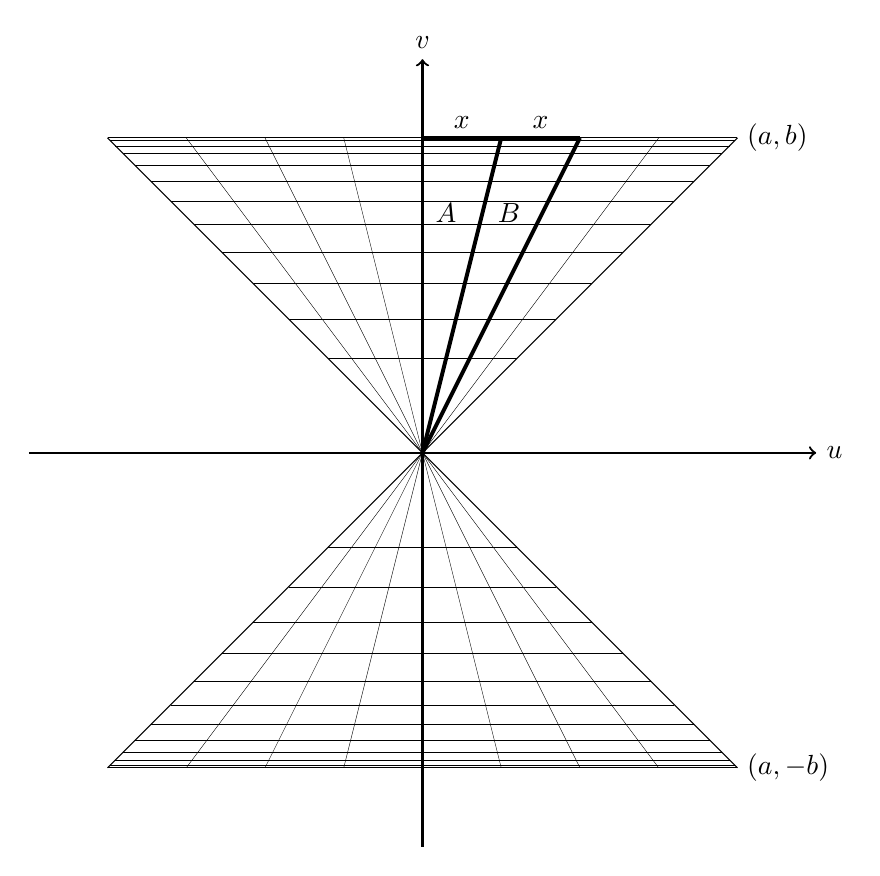
\begin{tikzpicture}
		% X - axis
		\draw[->,thick] (-5,0)--(5,0) node[right]{$u$};
		% Y - axis
		\draw[->,thick] (0,-5)--(0,5) node[above]{$v$};
		% Thick Lines
		\draw [line width=0.5mm] (0,0) -- (1,4);
		\draw [line width=0.5mm] (0,4) -- (1,4);
		\draw [line width=0.5mm] (1,4) -- (2,4);
		\draw [line width=0.5mm] (0,0) -- (2,4);
		\draw [line width=0.5mm] (0,0) -- (0,4);
		% Label the two areas 
		\node at (0.3,3.04) {$A$};
		\node at (1.1,3.04) {$B$};
		% Label the lengths as equivalent
		\node at (0.5,4.2) {$x$};
		\node at (1.5,4.2) {$x$};
		% Lines for the meridians right side
		\draw (-4,-4 ) -- (4,4);
		\draw [line width=0.05mm] (-3,-4 ) -- (3,4);
		\draw [line width=0.05mm] (-2,-4 ) -- (2,4);
		\draw [line width=0.05mm] (-1,-4 ) -- (1,4);
		\draw [line width=0.05mm] (0,-4 ) -- (0,4);
		\draw [line width=0.05mm] (1,-4 ) -- (-1,4);
		\draw [line width=0.05mm] (2,-4 ) -- (-2,4);
		\draw [line width=0.05mm] (3,-4 ) -- (-3,4);
		\draw (4,-4 ) -- (-4,4);
		\draw (-4,4 ) -- (4,4) node[right]{$(a,b)$};
		\draw (-4,-4 ) -- (4,-4) node[right]{$(a,-b)$};
		% Lines for the latitudes
		\draw [line width=0.05mm] (-3.965,3.965) -- (3.965,3.965);
		\draw [line width=0.05mm] (-3.9,3.9) -- (3.9,3.9);
		\draw [line width=0.05mm] (-3.8,3.8) -- (3.8,3.8);
		\draw [line width=0.05mm] (-3.65,3.65) -- (3.65,3.65);
		\draw [line width=0.05mm] (-3.45,3.45) -- (3.45,3.45);
		\draw [line width=0.05mm] (-3.2,3.2) -- (3.2,3.2);
		\draw [line width=0.05mm] (-2.9,2.9) -- (2.9,2.9);
		\draw [line width=0.05mm] (-2.55,2.55) -- (2.55,2.55);
		\draw [line width=0.05mm] (-2.15,2.15) -- (2.15,2.15);
		\draw [line width=0.05mm] (-1.7,1.7) -- (1.7,1.7);
		\draw [line width=0.05mm] (-1.2,1.2) -- (1.2,1.2);
		% Lines for the meridians left side
		\draw [line width=0.05mm] (-3.965,-3.965) -- (3.965,-3.965);
		\draw [line width=0.05mm] (-3.9,-3.9) -- (3.9,-3.9);
		\draw [line width=0.05mm] (-3.8,-3.8) -- (3.8,-3.8);
		\draw [line width=0.05mm] (-3.65,-3.65) -- (3.65,-3.65);
		\draw [line width=0.05mm] (-3.45,-3.45) -- (3.45,-3.45);
		\draw [line width=0.05mm] (-3.2,-3.2) -- (3.2,-3.2);
		\draw [line width=0.05mm] (-2.9,-2.9) -- (2.9,-2.9);
		\draw [line width=0.05mm] (-2.55,-2.55) -- (2.55,-2.55);
		\draw [line width=0.05mm] (-2.15,-2.15) -- (2.15,-2.15);
		\draw [line width=0.05mm] (-1.7,-1.7) -- (1.7,-1.7);
		\draw [line width=0.05mm] (-1.2,-1.2) -- (1.2,-1.2);
	\end{tikzpicture}
	\end{center}

	Using the solution to the differential equation we solved in part (b), we have the variable $v$ in terms of $\theta$. 

	% Display the variable v in terms of theta
	\begin{align*}
	v(\theta) & =
	\begin{cases}
	b\sqrt{\abs{\sin \theta}} & \text{for } 0 \leq \theta \leq \frac{\pi}{2}\\ -b\sqrt{\abs{\sin \theta}} & \text{for } -\frac{\pi}{2} \leq \theta < 0\\
	\end{cases}\\
	-\frac{\pi}{2} & \leq \theta \leq \frac{\pi}{2}\\
	\end{align*}

	See the following page for the coordinate $u(\varphi,\theta)$.

	\pagebreak

	Furthermore, this map projection is equal area, so we know that the areas $A$ and $B$ are equal. As they have the same height, the intervals, $x$, that each longitudinal area subtends must be equivalent to preserve area. Therefore, $x = \frac{\varphi}{\pi}$, and thus $u(\varphi,\theta)$ is  dependent upon $v(\theta)$, and $\varphi$. Hence the derivation of $u(\varphi,\theta)$ is from the area of the triangle $A$ or $B$.

	\begin{align*}
	Area_A & = \frac{1}{2}bh\\
	& = \frac{1}{2}\times \frac{\varphi}{\pi} {v(\theta)}\\
	& = \frac{v\varphi}{2\pi}\\
	\therefore u(\varphi,\theta) & = \frac{v\varphi}{2\pi}\\
	& = \frac{\varphi}{2\pi}b{\sqrt{\abs{\sin{\theta}}}}\\
	& = \frac{\varphi}{ab}b{\sqrt{\abs{\sin{\theta}}}}\\
	& = \frac{\varphi}{a}{\sqrt{\abs{\sin{\theta}}}}\\
	\\
	\therefore u(\varphi,\theta) & = \frac{\varphi}{a}{\sqrt{\abs{\sin{\theta}}}}\\
	-\pi & < \varphi \leq \pi\\
	\end{align*}

	The range of $\varphi$ incorporates the full rotation around the sphere, and its sign determines the sign of $u(\varphi,\theta)$, and thus we do not need to consider the piecewise branches of $v(\theta)$.
	

\end{enumerate}
\end{document}
